%
% $Id: $
%
%
% Compilar a .pdf con LaTeX (pdflatex)
% Es necesario instalar Beamer (paquete latex-beamer en Debian)
%

%
% Gr�ficos:
% Los gr�ficos pueden suministrarse en PNG, JPG, TIF, PDF, MPS
% Los EPS deben convertirse a PDF (usar epstopdf)
%

\documentclass{beamer}
\usetheme{Warsaw}
\usebackgroundtemplate{
\includegraphics[width=\paperwidth]{format/libresoft-bg-soft.png}}
\usepackage[spanish]{babel}
\usepackage[latin1]{inputenc}
\usepackage{graphics}
\usepackage{amssymb} % Simbolos matematicos

%\definecolor{libresoftgreen}{RGB}{162,190,43}
%\definecolor{libresoftblue}{RGB}{0,98,143}

%\setbeamercolor{titlelike}{bg=libresoftgreen}

%% Metadatos del PDF.
\hypersetup{
  pdftitle={Introduction to Libre Software / Master on Libre Software (URJC)},
  pdfauthor={Jesus M. Gonzalez-Barahona},
  pdfcreator={GSyC/LibreSoft, Universidad Rey Juan Carlos},
  pdfproducer=PDFLaTeX,
  pdfsubject={Introduction},
}
%%

%\includeonly{presentation}
\includeonly{introduction}


\begin{document}

\title{Introduction to Libre Software}
\subtitle{Master on Libre Software (URJC) \\
\url{http://master.libresoft.es}}
\author{Jesus M. Gonzalez-Barahona}
\institute{jgb@gsyc.es \\
GSyC/LibreSoft, Universidad Rey Juan Carlos}

\date{September 2010}

\frame{
\maketitle
\begin{center}

\includegraphics[width=6cm]{format/gsyc-urjc}
\end{center}
}


% Si el titulo o el autor se quieren acortar para los pies de p�gina
% se pueden redefinir aqu�:
%\title{Titulo corto}
%\author{Autores abreviado}


%% LICENCIA DE REDISTRIBUCION DE LAS TRANSPAS
\frame{
~
\vspace{3cm}

\begin{flushright}
\copyright 2000-2010 Jesus M. Gonzalez-Barahona. \\

Some rights reserved. \\
This document is distributed under the \\
Creative Commons Attribution-ShareAlike 3.0 licence, \\
available in \\
\url{http://creativecommons.org/licenses/by-sa/3.0}

The original version of this document is available at \\
\url{http://master.libresoft.es}
\end{flushright}
}
%%

%% presentation.tex
%%
%% Presentation of the course ``Master Thesis" of the Official Master on Libre Software (URJC)
%% http://master.libresoft.es
%%

%%---------------------------------------------------------------------
%%---------------------------------------------------------------------

\section{Presentation of the Master Thesis Course}

%%---------------------------------------------------------------

\begin{frame}
\frametitle{Administrative data}

\begin{itemize}
\item Both semesters, 12 ECTS credits
\item Teachers:
  \begin{itemize}
  \item Gregorio Robles (grex at gsyc.urjc.es)
  \item Jesus M. Gonzalez-Barahona (jgb at gsyc.urjc.es)
  \item Departamento de Sistemas Telem�ticos y Computaci�n (GSyC)
  \item Rooms 109 and 120 Departamental II (M�stoles campus)
  \item Room 103 Biblioteca (Fuenlabrada campus)
  \end{itemize}
\item Schedule: see Calendar
\item Sessions:
  \begin{itemize}
  \item Classroom 215, Aulario II, Fuenlabrada campus
  \end{itemize}
\item Moodle course (please, join it as soon as possible): \\
  \url{http://docencia.etsit.urjc.es/moodle/course/view.php?id=134}
\end{itemize}
\end{frame}

%%---------------------------------------------------------------

\begin{frame}
\frametitle{Goals}

Primary Goal: 
To apply the lessons and practices learned in this master
to a real problem

Secondary goal
To do it in one term

\end{frame}

%%---------------------------------------------------------------


\begin{frame}
\frametitle{Evaluation}

\begin{itemize}
\item 
\end{itemize}

\end{frame}

%%---------------------------------------------------------------

\begin{frame}
\frametitle{}

\begin{itemize}
\item 
\end{itemize}

\end{frame}

%%---------------------------------------------------------------

\begin{frame}
\frametitle{}

\begin{itemize}
\item 
\end{itemize}

\end{frame}

%%---------------------------------------------------------------

\begin{frame}
\frametitle{}

\begin{itemize}
\item 
\end{itemize}

\end{frame}


%%---------------------------------------------------------------

\begin{frame}
\frametitle{Some references}

\begin{itemize}
\item  \\
  \url{}
\item Introduction to libre software (book) \\
  \url{http://curso-sobre.berlios.de/introsobre}
\end{itemize}

\end{frame}

%% introduction.tex
%%
%% Introduction to the course ``Economic aspects'' of the
%%   Official Master on Libre Software (URJC)
%%   http://master.libresoft.es

%%---------------------------------------------------------------------
%%---------------------------------------------------------------------
\section{Introduction and motivation}

%%---------------------------------------------------------------

\begin{frame}
\frametitle{The growth of libre software (1)}

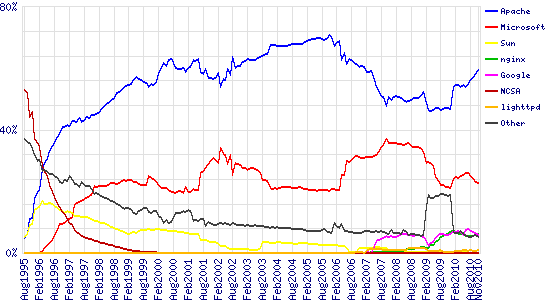
\includegraphics[height=6cm]{webservers-share-2010-11}

\begin{flushright}
Netcraft Survey, November 2010 \\
{\small \url{http://news.netcraft.com/archives/2010/11/05/november-2010-web-server-survey.html}}
\end{flushright}
\end{frame}

%%---------------------------------------------------------------

\begin{frame}
\frametitle{The growth of libre software (2)}

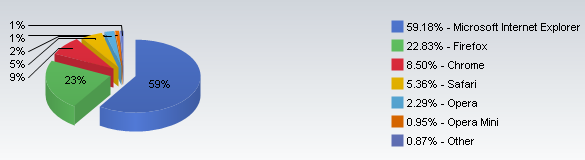
\includegraphics[height=3.5cm]{webbrowsers-share-2010-10}

\begin{flushright}
Net Market Share Report, October 2010 \\
{\small \url{http://www.netmarketshare.com/}}
\end{flushright}
\end{frame}

%%---------------------------------------------------------------

\begin{frame}
\frametitle{The growth of libre software (3)}

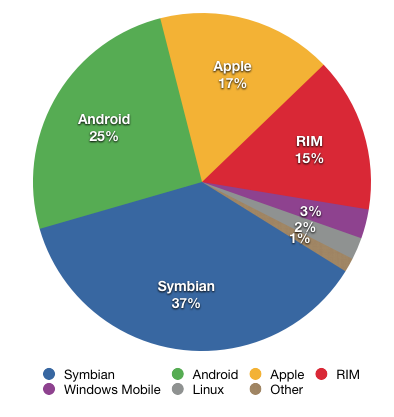
\includegraphics[height=5cm]{smartphone-share-gartner-2010-q3}

\begin{flushright}
Competitive Landscape: Mobile Devices, 3Q10 (Gartner)\\
Worldwide smartphone sales, 3rd Q 2010 \\
{\small \url{http://www.gartner.com/it/page.jsp?id=1466313}} \\
(graph from Wikimedia Commons)
\end{flushright}
\end{frame}


%%---------------------------------------------------------------

\begin{frame}
\frametitle{The adoption of libre software (1)}

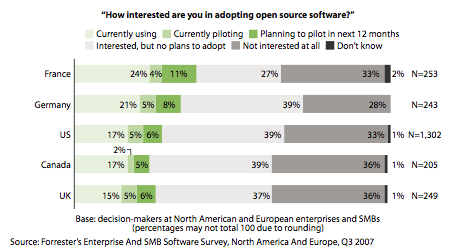
\includegraphics[height=5cm]{adoption-interest-forrester-2007-q3}

\begin{flushright}
Open Source Adoption: Notes From The Field \\
(Forrester, July 2008) \\
{\small \url{http://www.forrester.com/rb/Research/open_source_adoption_notes_from_field/q/id/46279/t/2}} 
\end{flushright}
\end{frame}

%%---------------------------------------------------------------

\begin{frame}
\frametitle{The adoption of libre software (2)}

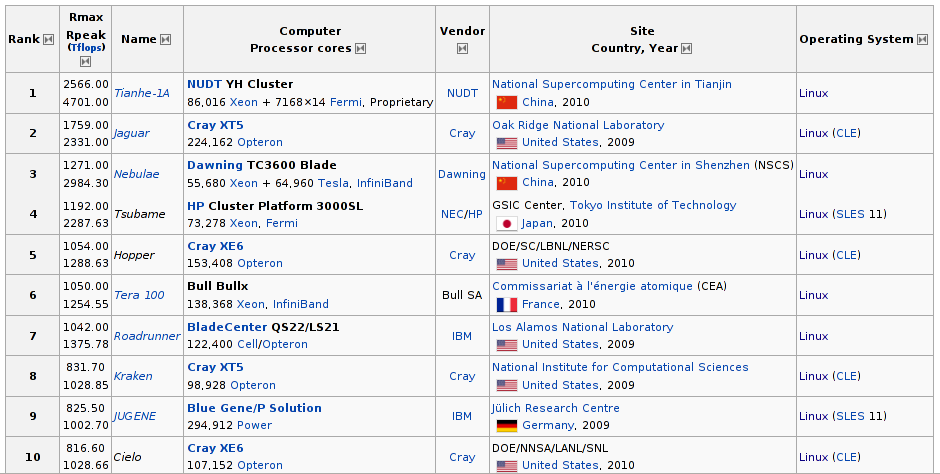
\includegraphics[height=6cm]{top-10-supercomputers-2010-11}

\begin{flushright}
36th TOP500 List (November 2010) \\
{\small \url{http://www.top500.org} \url{http://en.wikipedia.org/wiki/TOP500}} 
\end{flushright}
\end{frame}

%%---------------------------------------------------------------

\begin{frame}
\frametitle{The adoption of libre software (3)}

\begin{center}
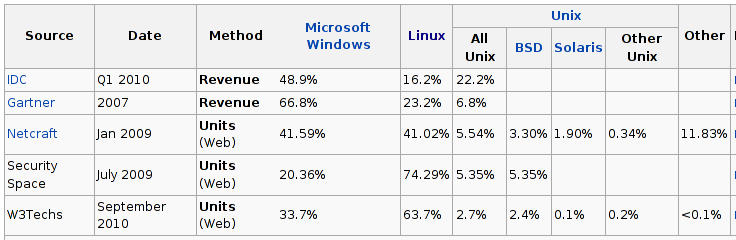
\includegraphics[height=4cm]{server-os-share-2010}
\end{center}

\begin{flushright}
Server market share, operating systems (Wikipedia) \\
{\footnotesize \url{http://en.wikipedia.org/wiki/Usage_share_of_operating_systems}} 
\end{flushright}
\end{frame}

%%---------------------------------------------------------------

\begin{frame}
\frametitle{The adoption of libre software (4)}

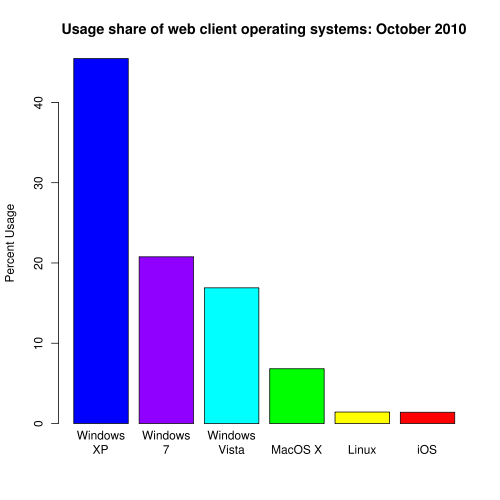
\includegraphics[height=6cm]{desktop-os-marketshare-2010-10}

\begin{flushright}
Usage share of web client operating systems \\
(Wikipedia, October 2010, median of usage studies) \\
{\small \url{http://en.wikipedia.org/wiki/Usage_share_of_desktop_operating_systems}} 
\end{flushright}
\end{frame}

\end{frame}



\end{document}
